\documentclass[11pt, envcountsect, aspectratio=169]{beamer}
\usepackage[utf8]{inputenc}
\usepackage[T1]{fontenc}
\usepackage{lmodern}
\usepackage[english]{babel}
\usepackage{amsmath}
\usepackage{amsfonts}
\usepackage{amssymb}
\usepackage{graphicx}
\usepackage{grffile}
\usetheme{default}

\newenvironment<>{proposition}[1][\undefined]{%
\begin{actionenv}#2%
\ifx#1\undefined%
   \def\insertblocktitle{Theorem}%
\else%
   \def\insertblocktitle{Theorem ({\em#1})}%
\fi%
\par%
\usebeamertemplate{block begin}\em}
{\par\usebeamertemplate{block end}\end{actionenv}}

\begin{document}

\author{José C. Oliveira}
\title{3.5 Multinomial Opinions}
%\subtitle{}
%\logo{}
%\institute{}
%\date{}
%\subject{}
%\setbeamercovered{transparent}
%\setbeamertemplate{navigation symbols}{}
\begin{frame}[plain]
	\maketitle
\end{frame}

\section*{Outline}
\begin{frame}{Summary}
    \tableofcontents
\end{frame}

\section{3.5.1 The Multinomial Option Representation}

\begin{frame}[allowframebreaks]{3.5.1 The Multinomial Opinion Representation}
    \begin{block}{Definition 3.4 (Multinomial Opinion)}
        Let $\mathbb{X}$ be a domain larger than binary, i.e. so that $k = |\mathbb{X}| > 2$. Let $X$ be a random variable in $\mathbb{X}$. A multinomial opinion over the random variable $X$ is the ordered triplet $\omega_X = (\mathbf{b}_X, u_X , \mathbf{a}_X)$ where
        \begin{itemize}
            \item $\mathbf{b}_X$ is a belief mass distribution over $X$,
            \item $u_X$ is the uncertainty mass which represents the vacuity of evidence,
            \item $\mathbf{a}_X$ is a base rate distribution over $\mathbb{X}$,
        \end{itemize}
        and the multinomial additivity requirement of Eq.(2.6) is satisfied.
    \end{block} ~\\

    A multinomial opinion has $(2k - 1)$ degrees of freedom.
\end{frame}

\begin{frame}{3.5.1 The Multinomial Opinion Representation}
    The projected probability distribution of multinomial opinions is defined by:
    \begin{equation}\label{eq:multinomial_projected_probability}\tag{3.12}
       	\mathbf{P}_X(x) = \mathbf{b}_X(x) + \mathbf{a}_X(x) u_X,\ \forall x \in \mathbb{X}\text{.}
    \end{equation}

%    The variance of multinomial opinions is expressed as
%    \begin{equation}\tag{3.13}
%       	\mathrm{Var}_X = \dfrac{\mathbf{P}_X(x)(1 - \mathbf{P}_X(x)u_X)}{W + u_X},
%    \end{equation}
%    where $W$ denotes non-informative prior weight, which must be set to $W = 2$.
\end{frame}

\begin{frame}{3.5.1 The Multinomial Opinion Representation}
    \begin{figure}
        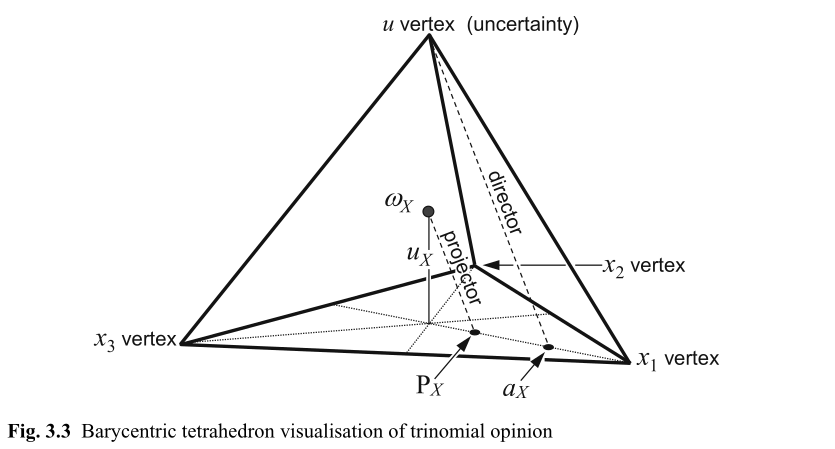
\includegraphics[width = \textwidth]{images/fig3.3.png}
    \end{figure}
\end{frame}

\section{3.5.2 The Dirichlet Multinomial Model}

\begin{frame}{3.5.2 The Dirichlet Multinomial Model}
    \begin{block}{Definition 3.4 (Dirichlet Probability Density Function)}
    	Let $\mathbb{X}$ be a domain consisting of $k$ mutually disjoint values. Let $\alpha_X$ represent the strength vector over the values of $\mathbb{X}$, and let $\mathbf{p}_X$ denote the probability distribution over $\mathbb{X}$. With $\mathbf{p}_X$ as a $k$-dimensional variable, the Dirichlet PDF denoted $\mathrm{Dir}(\mathbf{p}_X, \alpha_{X})$ is expressed as:
    	\begin{equation}\tag{3.14}
    		\mathrm{Dir}(\mathbf{p}_X, \alpha_X) = \dfrac{\Gamma\left(\sum\limits_{x \in \mathbb{X}} \alpha_X(x)\right)}{\prod\limits_{x \in \mathbb{X}} \Gamma(\alpha_X(x))} \prod\limits_{x \in \mathbb{X}} \mathbf{p}_X(x)^{(\alpha_X(x)-1)} \text{, where } \alpha_X(x) \geq 0\text{,}
    	\end{equation}
    	with the restrictions that $\mathbf{p}_X(x) \neq 0$ if $\alpha_X(x) < 1$.
    \end{block}
\end{frame}

\begin{frame}{3.5.2 The Dirichlet Multinomial Model}
    \framesubtitle{The evidence representation of the Dirichlet PDF}
    The evidence representation of the Dirichlet PDF is denoted by $\mathrm{Dir}^{\mathrm{e}}_X(\mathbf{p}_X, \mathbf{r}_X, \mathbf{a}_X)$, where the total strength $\alpha_X(x)$ for each value $x \in \mathbb{X}$ can be expressed as
    \begin{equation}\tag{3.15}
        \alpha_X(x) = \mathbf{r}_X(x) + \mathbf{a}_X(x)W\text{, where }\mathbf{r}_X(x) \geq 0\ \forall x \in \mathbb{X}\text{.}
    \end{equation}

    \begin{itemize}
        \item $\mathbf{r}_X(x)$ is the evidence for outcome $x \in \mathbb{X}$.
        \item $\mathbf{a}_X$ is the base rate distribution.
        \item $W$ is the non-informative prior weight.
    \end{itemize}
\end{frame}

\begin{frame}{3.5.2 The Dirichlet Multinomial Model}
    \framesubtitle{The evidence representation of the Dirichlet PDF}
    The expected distribution over $\mathbb{X}$ can be written as
    \begin{equation}\label{eq:dirithlet_expected_probability}\tag{3.17}
        \mathbf{E}_X(x) = \dfrac{\alpha_X(x)}{\sum\limits_{x_j \in \mathbb{X}} \alpha_X(x_i)} = \dfrac{\mathbf{r}_X(x) + \mathbf{a}_X(x)W}{W + \sum\limits_{x_j \in \mathbb{X}} \mathbf{r}_X(x_j)}\ \forall x \in \mathbb{X}.
    \end{equation}

%    The variance of the Dirichlet is defined by
%    \begin{equation}\tag{3.18}
%        \mathrm{Var}_X(x) = \dfrac{\mathbf{P}_X(x)(1 - \mathbf{P}_X(x))}{W + u_X}\text{.}
%    \end{equation}
\end{frame}

\section{3.5.3 Visualizing Dirichlet Probability Density Functions}

\begin{frame}{3.5.3 Visualizing Dirichlet Probability Density Functions}
    Dirichlet PDFs over ternary domains are the largest that can be practically visualized.

    Example: Urn with balls with three different markins: $x_1$, $x_2$ and $x_3$.

    \begin{columns}
        \begin{column}{4.8cm}
            \begin{figure}
                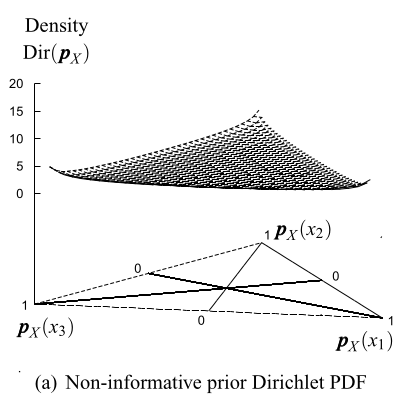
\includegraphics[scale=0.37]{images/fig3.4.a.png}
            \end{figure}
        \end{column}
        \begin{column}{5.8cm}
           $\mathbf{a}_X(x) = 1/k = 1/3$

           $\mathbf{r}_X(x_1) = \mathbf{r}_X(x_1) =\mathbf{r}_X(x_1) = 0$

           $\mathbf{E}_X(x_1) = 1/3$
        \end{column}
    \end{columns}
\end{frame}

\begin{frame}{3.5.3 Visualising Dirichlet Probability Density Functions}
    Dirichlet PDFs over ternary domains are the largest that can be practically visualized.

    Example: Urn with balls with three different markins: $x_1$, $x_2$ and $x_3$.

    \begin{columns}
        \begin{column}{4.8cm}
            \begin{figure}
                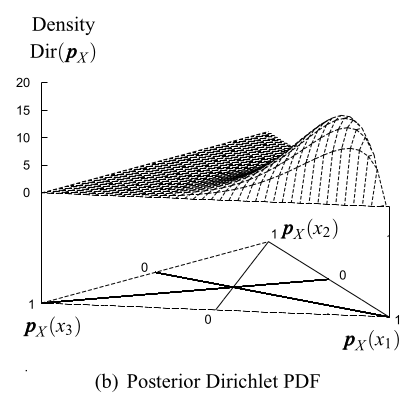
\includegraphics[scale=0.37]{images/fig3.4.b.png}
            \end{figure}
        \end{column}
        \begin{column}{5.8cm}
            $\mathbf{a}_X(x) = 1/k = 1/3$

            $\mathbf{r}_X(x_1) = 6$

            $\mathbf{r}_X(x_2) = 1$

            $\mathbf{r}_X(x_3) = 1$

            $\mathbf{E}_X(x_1) = 2/3$
        \end{column}
    \end{columns}
\end{frame}

\section{3.5.4 Coarsening Example: From Ternary to Binary}

\begin{frame}{3.5.4 Coarsening Example: From Ternary to Binary}
    Same case as before, but $x_1 = x_1$ and $\overline{x}_1 = \{x_2, x_3\}$

    \begin{figure}
        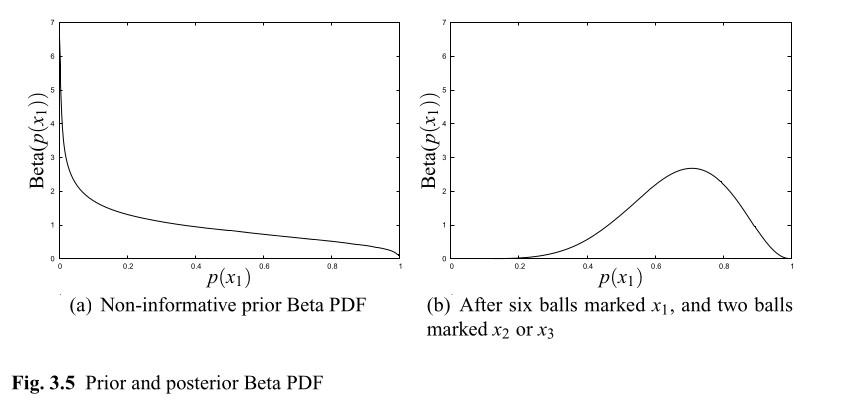
\includegraphics[scale=0.37]{images/fig.3.5.png}
    \end{figure}

    $\mathbf{E}_X(x_1) = 2/3$, same as before.
\end{frame}

\section{3.5.5 Mapping Between Multinomial Opinion and Dirichlet PDF}

\begin{frame}{3.5.5 Mapping Between Multinomial Opinion and Dirichlet PDF}
    \framesubtitle{Requirements}

    \begin{equation}\tag{3.19}
        \mathbf{P}_X = \mathbf{E}_X
    \end{equation}

    \begin{equation}\tag{3.21}
        \sum\limits_{x \in \mathbb{X}} \mathbf{r}_X(x) \longrightarrow \infty \Rightarrow \sum\limits_{x \in \mathbb{X}} \mathbf{b}_X(x) \longrightarrow 1
    \end{equation}

    \begin{equation}\tag{3.22}
        \sum\limits_{x \in \mathbb{X}} \mathbf{r}_X(x) \longrightarrow \infty \Rightarrow u_X = 0
    \end{equation}
\end{frame}

\begin{frame}{3.5.5 Mapping Between Multinomial Opinion and Dirichlet PDF}
    \begin{block}{Definition 3.6 ((Mapping: Multinomial Opinion $\leftrightarrow$ Dirichlet PDF)}
        \emph{} Let $\omega_X = (\mathbf{b}_X, u_X, \mathbf{a}_X)$ be a multinomial opinion and let $\mathrm{Dir}^\mathrm{e}_X(\mathbf{p}_X, \mathbf{r}_X, \mathbf{a}_X)$ be a Dirichlet PDF, both over the same variable $X \in \mathbb{X}$. These are equivalent through the following mapping,
        \begin{equation}\tag{3.23}
            \begin{split}
                & \forall x \in \mathbb{X} \\
                & \begin{cases}
                    \mathbf{b}_X(x) & = \dfrac{\mathbf{r}_X(x)}{W + \sum\limits_{x_i \in \mathbb{X}} \mathbf{r}_X(x_i)} \\
                    u_X & = \dfrac{W}{W + \sum\limits_{x_i \in \mathbb{X}} \mathbf{r}_X(x_i)}
                \end{cases} \Leftrightarrow
                \begin{cases}
                    \begin{cases}
                        \mathbf{r}_X(x) = \dfrac{W \mathbf{b}_X(x)}{u_X} \\
                        1 = u_X = \sum\limits_{x_i \in \mathbb{X}} \mathbf{b}_X(x_i)
                    \end{cases} & \text{if } u_X \neq 0 \\
                    \begin{cases}
                        \mathbf{r}_X(x) = \mathbf{b}_X(x) \cdot \infty \\
                        1 = \sum\limits_{x_i \in \mathbb{X}} \mathbf{b}_X(x_i)
                    \end{cases} & \text{if } u_X \neq 0
                \end{cases}
            \end{split}
        \end{equation}
    \end{block}
\end{frame}

\section{3.5.6 Uncertainty-Maximisation}

\begin{frame}{3.5.6 Uncertainty-Maximisation}

\end{frame}

\end{document}

